\documentclass[fleqn]{article}
\usepackage[margin=1.5cm]{geometry}   % shrink margins
\usepackage{amsmath}    % math equation environments
% \usepackage{amssymb}    % math symbols such as natural numbers N.
\usepackage{tikz}	% for diagrams
\usepackage{algorithm}
\usepackage[noend]{algpseudocode}
\usepackage{adjustbox}	% align enumerations containing tall objects to top. Usage: \item\adjustbox{valign=t}{...}
% \usepackage{centernot}	% centers not symbol. Usage: \centernot{...}

% paragraph indentation within enumerations
\usepackage{enumitem}
\setlist{parsep=4pt,listparindent=\parindent}

\tikzset{
	vertex/.style args = {#1}{circle, draw=#1!80, fill=#1!20},
	vertex/.default = blue,
}

\title{Data Structures \\
\large Theoretical Homework 5}
\author{Abraham Murciano}

\begin{document}

\maketitle

\begin{enumerate}

	\item % 1
	\begin{enumerate}
		\item % a
		\begin{enumerate}
			\item % i
			The graph shown in figure \ref{fig:connected_bipartate_graph} is connected and bipartite.
			\begin{figure}[h]
				\centering
				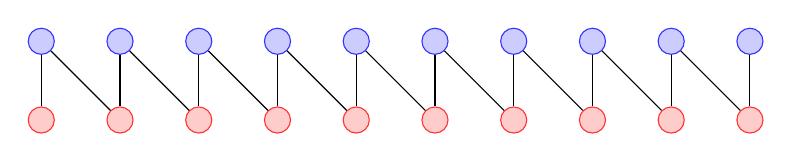
\begin{tikzpicture}
					\foreach \x in {0,...,9} {
						\node[vertex={blue}] (top_\x) at (\x, 0) {};
					}
					\foreach \x in {0,...,9} {
						\node[vertex={red}] (bottom_\x) at (\x, -1) {};
					}
					\foreach \x in {0,...,9} {
						\draw (top_\x) -- (bottom_\x);
					}
					\foreach \x [evaluate=\x as \xplusone using int(\x + 1)] in {0,...,8} {
						\draw (top_\x) -- (bottom_\xplusone.north west);
					}
				\end{tikzpicture}
				\caption{Connected bipartite graph}
				\label{fig:connected_bipartate_graph}
			\end{figure}
								
			\item % ii
			The graph in figure \ref{fig:disconnected_bipartate_graph} is disconnected as well as bipartite. In fact any graph with no edges is bipartite.
			\begin{figure}[h]
				\centering
				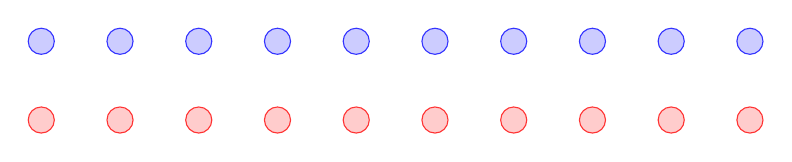
\begin{tikzpicture}
					\foreach \x in {0,...,9} {
						\node[vertex={blue}] (top_\x) at (\x, 0) {};
					}
					\foreach \x in {0,...,9} {
						\node[vertex={red}] (bottom_\x) at (\x, -1) {};
					}
				\end{tikzpicture}
				\caption{Disconnected bipartite graph}
				\label{fig:disconnected_bipartate_graph}
			\end{figure}
		\end{enumerate}

		\item % b
		This is an algorithm which will tell us if the graph \(G = (V, E)\) is bipartite or not. It attempts to colour each connected component with only two colours, and if it fails, then \(G\) is not bipartite.
		\begin{algorithmic}[1]
			\Function{Bipartite}{graph $G(V, E)$}
				\ForAll{\(v \in V\)} \Comment{Mark each vertex as not visited}
					\State \(v\).colour = NULL
				\EndFor
				\ForAll{\(v \in V\)}
					\If{\(v\).colour == NULL} \Comment{\(v\) is part of an unvisited connected component}
						\If{ColourConnectedComponent(\(v\)) == false}
							\State \Return false \Comment{We were unable to colour this component with two colours}
						\EndIf
					\EndIf
				\EndFor
				\State \Return true
			\EndFunction
			\\
			\Function{ColourConnectedComponent}{vertex $v$, colour $c$ = BLUE}
			\State \(v\).colour = \(c\)
			\If{c == BLUE}
				\State OppositeColour = RED
			\Else
				\State OppositeColour = BLUE
			\EndIf
				\ForAll{\(u\) adjacent to \(v\)}
					\If{\(u\).colour == \(v\).colour} \Comment{If a vertex is connected to another of the same colour,}
						\State \Return false \Comment{then it is not bipartite}
					\ElsIf{\(u\).colour == NULL}
						\State ColourConnectedComponent(\(u\), OppositeColour) \Comment{Recursively colour all \(v\)'s neigbours}
					\EndIf
				\EndFor
				\State \Return true
			\EndFunction
		\end{algorithmic}
	\end{enumerate}

	\item % 2
	\begin{enumerate}
		\item % a
		In order to aid the upcoming definitions, we will define a \textbf{path} from \(v\) to \(u\) as a sequence of edges \(P\) whose first edge is of the form \(\{v, x\}\) and its last edge is of the form \(\{y, u\}\), and each other edge in \(P\) shares one of its vertices with the previous edge in the sequence and shares its other vertex with the next edge in the sequence.
		\begin{enumerate}
			\item % i
			A \textbf{directed graph} \(G(V, E)\) is a graph whose set of edges \(E\) is a set of \textit{ordered} pairs of vertices.

			\item % ii
			A \textbf{connected graph} \(G(V, E)\) is a graph such that for all two vertices \(v, u \in V\), there exists a path from \(v\) to \(u\).

			\item % iii
			An \textbf{acyclic graph} \(G(V, E)\) is a graph such that for all adjacent vertices \(v, u \in V\), all paths from \(v\) to \(u\) contain the edge \(\{v, u\}\).
		\end{enumerate}

		\item % b
		\begin{algorithmic}[1]
			\Function{MaximalOutDegree}{graph $G(V, E)$}
				\State HighestOutDegree = 0
				\For{\(i = 0\) to \(|V| - 1\)}
					\State OutDegree = 0
					\For{\(j = 0\) to \(|V| - 1\)}
						\State OutDegree += Adjacent[\(i\)][\(j\)] \Comment{If the \(i^{\text{th}}\) and \(j^{\text{th}}\) vertices are adjacent, increment OutDegree}
					\EndFor
					\If{OutDegree \(>\) HighestOutDegree}
						\State HighestOutDegree = OutDegree
					\EndIf
				\EndFor
				\State \Return HighestOutDegree
			\EndFunction
		\end{algorithmic}

		The complexity of this function is \(\Theta(|V|^2)\), since we must check every single possible edge in the adjacency matrix, and there are \(|V|^2\) elements in the matrix.
	\end{enumerate}

	\item % 3
	In figure \ref{fig:cycle_BFS_before_DFS} below, if a Depth First Search (DFS) algorithm was used to find cycles, it may occur that the algorithm would begin at node 0, then then reach node 1, and at that point it may choose to either continue to node 2 or to node 6. If the algorithm decided to take the path to node 2, it would continue onwards until reaching node 5, and only afterwards backtrack to node 1 in order to continue on the path to 6, after which it would again reach node 0 and proclaim the graph cyclic.

	However if a Breadth First Search (BFS) algorithm was employed, and it too began at node 0, the first two nodes it would find would be nodes 1 and 6. Then at the very next step it would find node 2 as well as the already visited nodes 1 and 6, therefore immediately concluding that the graph is cyclic.
	\begin{figure}[h]
		\centering
		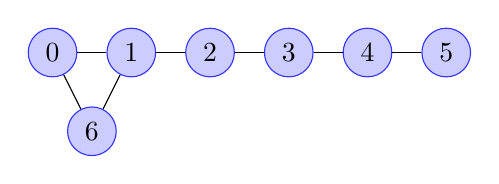
\begin{tikzpicture}
			\node[vertex] (node_0) at (0, 0) {0};
			\foreach \x [evaluate=\x as \xminusone using int(\x - 1)] in {1,...,5}{
				\node[vertex] (node_\x) at (\x, 0) {\x};
				\draw (node_\x) -- (node_\xminusone);
			}
			\node[vertex] (node_6) at (0.5, -1) {6};
			\draw (node_0) -- (node_6) -- (node_1);
		\end{tikzpicture}
		\caption{graph where BFS discovers a cycle before DFS}
		\label{fig:cycle_BFS_before_DFS}
	\end{figure}

	\item % 4
	The Following algorithm will return the number of shortest paths from a source node \(s\) to a destination node \(d\). It extends the Breadth First Search algorithm and achieves a run time complexity of \(\Theta(|V| + |E|)\).
	\begin{algorithmic}[1]
		\Function{CountShortestPaths}{graph \(G(V, E)\), vertex \(s\), vertex $d$}
			\ForAll{\(v \in V\)}
				\State \(v\).distance = \(\infty\)
				\State \(v\).count = 0
			\EndFor
			\State \(s\).distance = 0
			\State \(s\).count = 1
			\State Queue = \(\phi\)
			\State Queue \(\leftarrow s\)
			\While{Queue \(\neq \phi\)}
				\State \(v \leftarrow\) Queue
				\If{\(v\).distance \(\geq d\).distance}
					\State break
				\EndIf
				\ForAll{\(u\) adjacent to \(v\)}
					\If{\(u\).distance == \(\infty\)}
						\State \(u\).distance = \(v\).distance + 1
						\State \(u\).count = \(v\).count
						\State Queue \(\leftarrow u\)
					\ElsIf{\(u\).distance == \(v\).distance + 1}
						\State \(u\).count += \(v\).count
					\EndIf
				\EndFor
			\EndWhile
			\State \Return \(d\).count
		\EndFunction
	\end{algorithmic}

	\item % 5
	Given a set of \(N\) students and a set of pairs, where a pair \((i,j)\) means that student \(j\) copied the homework solution from student \(i\):
	\begin{enumerate}
		\item % a
		To find the set of students who did not copy from anyone, a graph can be built using an adjacency list. Each student would be represented by a vertex, and each edge \(a, b\) would indicate that student \(a\) copied from student \(b\). Once this graph is built, the students who did noy copy can be found as follows. The complexity of this algorithm is \(\Theta(|N|)\).
		\begin{algorithmic}[1]
			\State set \(S\) \Comment{\(S\) will store all the students who did not copy}
			\ForAll{\(v \in V\)}
				\If{edges[\(v\)] is empty}
					\State Insert \(v\) into \(S\)
				\EndIf
			\EndFor
		\end{algorithmic}

		\item % b
		To find the set of students whom nobody copied from, a graph can be built similarly to part (a), with one difference. Each edge \(a, b\) would indicate that student \(b\) copied from student \(a\). The algorithm and complexity would be exactly the same.

		\item % c
		To find the set of students who copied from a specific student, we can build a graph using an adjacency list, where each edge \((a, b)\) represents that student \(b\) copied from student \(a\), we can use the following algorithm. The complexity is \(\Theta(|N|)\).
		\begin{algorithmic}[1]
			\Function{StudentsWhoCopiedFrom}{student $s$}
				\State mark \(s\) as visited
				\ForAll{\(v\) adjacent to \(s\)}
					\If{\(v\) was not visited}
						\State Result.insert(\(v\))
						\State Result.union(\Call{StudentsWhoCopiedFrom}{$v$})
					\EndIf
				\EndFor
			\EndFunction
		\end{algorithmic}

		\item % d
		The question is not very clear. If my understanding of it is correct, then we would have to find the largest strongly connected component, complexity of which is \(\Theta(N + |E|)\)
	\end{enumerate}

	\item % 6
	\begin{enumerate}
		\item % a
		Run the Strongly Connected Component algorithm on the graph to find am acyclic component graph, then go through each vertex of the acyclic component graph, and check the in degree of that vertex. If there is exactly one vertex with an in degree of 0, then return any vertex from within that vertex. Otherwise, there is no root.
		
		\item % b
		If there is exactly one vertex in the acyclic component graph with an in degree of zero, then all the other vertices can be reached. Since the graph is acyclic, then they can all be reached from the vertex with the in degree of zero. Therefore any vertex within the strongly connected component of that vertex is a valid root.

		However if there is more than one vertex with an in degree of zero, then each of those vertices is unreachable from the others, hence none of them can be a root.
	\end{enumerate}

	\item % 7
	\begin{tabular}{||c||c|c|c|c|c|c||}
		\hline
		Vertex & \multicolumn{2}{c|}{Step 1} & \multicolumn{2}{c|}{Step 2} & \multicolumn{2}{c||}{Step 3} \\
		& \(d\) & \(\pi\) & \(d\) & \(\pi\) & \(d\) & \(\pi\) \\
		\hline
		A & 0 			& NULL & 0	& NULL	& \\
		B & \(\infty\) 	& NULL & 7	& A		& \\
		C & \(\infty\) 	& NULL & 8	& A		& \\
		D & \(\infty\) 	& NULL & 0	& NULL	& 12	& B\\
		E & \(\infty\) 	& NULL & 0	& NULL	& 9		& B\\
		F & \(\infty\) 	& NULL & 11	& A		& 
	\end{tabular}

\end{enumerate}
    
\end{document}
